\section{Use of Latin Hypercube in ecological studies}\label{Studies}
The importance of sensitivity and uncertainty analyses in the development 
and use of ecological models is widely recognized. Searching for the terms
``Sensitivity Analysis, Uncertainty Analysis or Parameter Space
Exploration'' in the Web of Knowledge reports 1199 papers in eight major
journals (see fig. \ref{fig:wok} and legend for details) since 1971, 
with 31650 total
citations. However,
most of these papers rely on full and individual parameter space
exploration, which, as discussed in section \ref{Sampling}, are not
optimal. When restricting those results with the keywords ``Latin Hypercube,
MCMC, Markov, Monte Carlo'', just 120 works show up in the results. Of 
% Gibbs Sampler - Incluir
those, only 13 (about $1\%$) use Latin Hypercube Sampling 
\cite{Berthaume12, Confalonieri10, Meyer07, Tiemeyer07, Xu05,
Moore04, Shirley03, Duchesne03, Reed84, Marino08, Nathan01, Hamilton10,
Lovvorn96}. There are also relevant examples of LHS use in other
journals \cite{Estill12, Fisher10, Thebault10}.

Also, many of these papers did not explicitly take into account the
correlations between parameters. Those who did used mostly Iman and 
Conover's method \cite{ImanConover82}. 

\begin{figure}[htpb]
		\begin{center}
				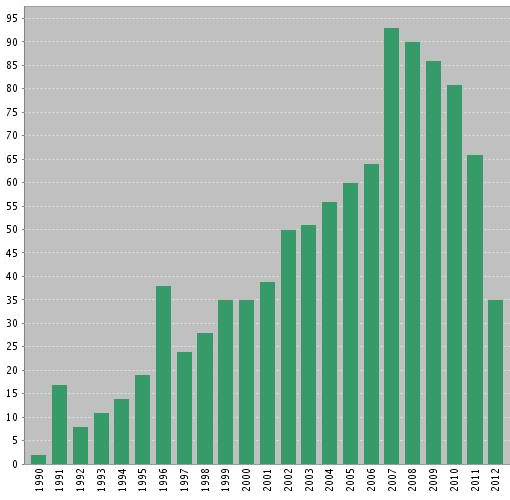
\includegraphics[width=263px]{fig/wok.png}
				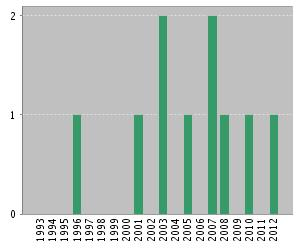
\includegraphics[width=243px]{fig/lhs.png}
		\end{center}
		\caption{Top: Number of papers per year since 1990 
		containing the topics ``Sensitivity 
		Analysis, Uncertainty Analysis or Parameter Space Exploration'' 
		in the journals American Naturalist, Ecology, Journal of 
		Ecology, Oikos, Oecologia, Ecological Modelling, 
		Ecology Letters, Journal of Theoretical Biology as reported by
		Thomson Reuter's Web of Knowledge.
		Bot: Restriction of the search above to the keywords ``Latin
		Hypercube''.
		Search conducted 18.06.2012,
		14h GMT.}
		\label{fig:wok}
\end{figure}

These works have used Latin Hypercubes typically from 10 to 30 dimensions,
but ranging from 6 to 143 \cite{Berthaume12},
and the number of
simulations ranged from 19 \cite{Nathan01} to 2000 \cite{Tiemeyer07}. 
Also, these works are from varied areas within ecology: applied plant 
ecology \cite{Confalonieri10, Tiemeyer07}, species richness 
\cite{Hamilton10}, epidemiology \cite{Shirley03} and food chain analysis
\cite{Duchesne03}, stressing that the method is useful on varied 
problems.
